\documentclass[10pt]{article}
\usepackage[margin=0.85in]{geometry}
\usepackage{amsmath,amssymb}
\usepackage{booktabs}
\usepackage{graphicx}
\usepackage{enumitem}
\usepackage[font=small,labelfont=bf]{caption}
\usepackage{hyperref}
\setlist{itemsep=1pt,topsep=3pt}
\setlength{\parskip}{4pt}
\setlength{\parindent}{0pt}
\emergencystretch=3em
\graphicspath{{figs/}}

\title{Challenge Problem 2 (City Zoning):\\ What made it hard, what we did, and what we learned}
\author{Pradyumnan Raghuveeran \and Rasmus Makela}
\date{November 13, 2026}

\begin{document}
\maketitle

\section{The problem, and where we ended up}

We had to hand in 100 layouts of a $7\times7$ city, where each cell is Residential, Industrial, Commercial, a Park or an Office. Four advisors (Wellness, Tax, Transportation, Business) rate a layout between 0 and 1, but we are never told how. A layout only counts if \emph{all four} give it at least 0.75. Among the layouts that count, each earns the average fraction of cells in which it differs from its 10 most similar neighbours, and the sum is divided by 100. So we need many valid layouts that are spread far apart, and a single invalid one throws away its whole contribution. We were given 500{,}000 layouts, but only 5{,}000 ratings per advisor.

Our final submission is \texttt{S22}: 100 distinct layouts, all valid under advisor rules that we recovered exactly (Section~3.2), with diversity score $38048/49000 = \mathbf{0.7764897959}$. Our earlier upload S19 scored $0.7753061224$ and matched our prediction to the last digit, which is how we know the predictions can be trusted. We held S22 back until the end of the competition, so its returned score was not known when we wrote this.

\begin{figure}[h]
\centering
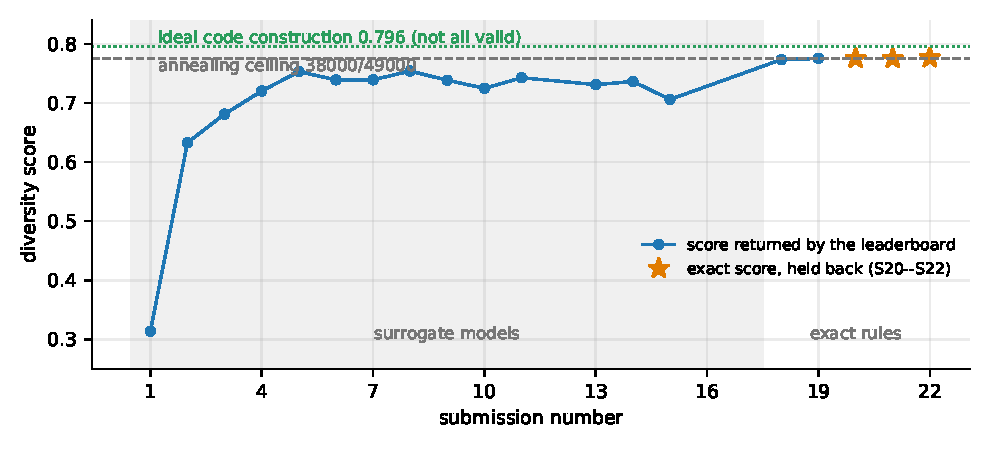
\includegraphics[width=0.85\linewidth]{fig1_progress.pdf}
\caption{Every score we received (blue) and the three sets we held back (orange). The jump after submission 17 is the point where we stopped guessing the advisors and recovered their formulas; the last step above the dashed line comes from the fixed-core idea in Section~3.3.}
\end{figure}

\section{What made it hard}

\textbf{We could not see the objective.} With 1\% of the labels, no layout in the data is rated valid by all four advisors, and Wellness and Tax pull in opposite directions: Wellness likes parks, Tax charges for them. On the 51 grids rated by both, none passed both.

\textbf{Validity is all or nothing, and we get almost no feedback.} We could upload five times per day and each upload returns one number. A model that is 95\% sure about each layout still gets around five of a hundred wrong, and each wrong layout costs about $0.0075$. We found out the hard way that a good-looking prediction is not a valid layout.

\textbf{The data is the wrong place to search.} The layouts that look valid are all alike. The best 100 of them score only $0.32$ even if every one is valid. A good score needs layouts that are not in the data, which is exactly where a trained model is least reliable.

\textbf{It is a packing problem on top of that.} Valid layouts need about 7--9 parks and almost exactly 10 residential cells (Figure~\ref{fig:comp}), so they all live in a narrow corner of the space. We still need 100 of them whose ten nearest neighbours are all far away.

\section{What we did}

\subsection{First attempt: learn the advisors}
We started the usual way. We trained gradient-boosted trees on counts, adjacency and distance features, and CNNs with rotation and flip augmentation, then blended them (held-out $R^2$ of 0.91 for Wellness, 0.98 for Tax, 0.97 for Transportation and 0.99 for Business). We then used simulated annealing on the whole set of 100 layouts, requiring each layout to have a high predicted probability of being valid. This took us from $0.31$ (layouts taken from the data, S1) to $0.63$ with generated layouts (S2) and finally to $0.754$ (S8, which was fully valid). Then it stopped. Loosening the safety margin produced invalid layouts faster than it bought diversity. To test this we submitted a certified set with 8 deliberately risky layouts swapped in (S15): 6 of the 8 were invalid, so the valid region does not extend beyond what the models believed.

\subsection{The turning point: the advisors are exact integer formulas}
Two things we noticed changed the project. First, the label values sit on an exact grid ($k/999$) with many identical values. The labels are a quantile transform of an \emph{integer} score (Figure~\ref{fig:labels}), so the advisors are deterministic, and predicting the transformed target already improved every model. Second, we had assumed an advisor treats a layout and its rotation or flip alike. That was wrong: they care about direction, for example ``a park directly to the left of a residential cell''. Our augmented CNNs had been averaging this signal away, which is why every model family hit the same error floor. Once we split each adjacency term by direction, the residuals collapsed, and we could fit each advisor as a sum of simple integer terms and accept a formula only if every label level mapped to a single score. For example (with $n_X$ the number of cells of type $X$):
\begin{align*}
\text{Tax} &= 10n_R+3n_C-20n_P-2\,\#(R\text{--}I\text{ adjacent})+8\#(P\text{ left of }R)+3\#(P\text{ right of }R)\\
&\quad+10\#(P\text{ above }R)+3\#(P\text{ below }R).
\end{align*}
Wellness, Transportation and Business are similar (nearest-distance terms plus directional adjacencies; Business is a labour-market rule with a $\max(0,\cdot)$). They reproduce all 20{,}000 labels and the score of every one of our 13 earlier submissions to the integer, including which advisor each failed layout broke (mostly Tax). A layout is valid exactly when the four integers reach $[70,\,17,\,-187,\,-1155]$.
From here on validity was a fact, not a probability, and the surrogate models were no longer needed.

\begin{figure}[h]
\centering
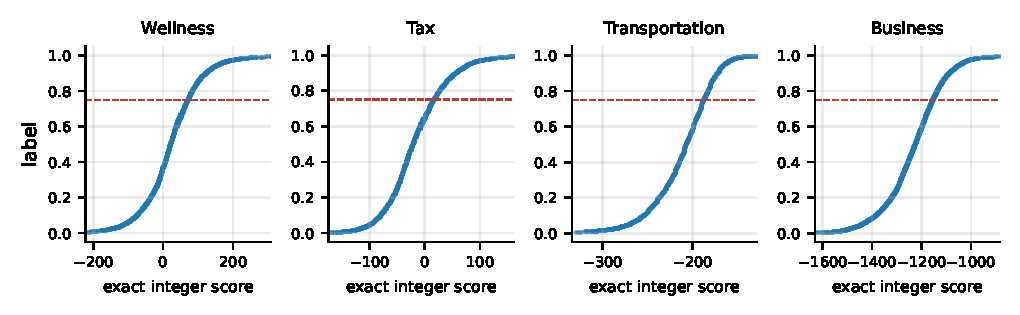
\includegraphics[width=0.95\linewidth]{fig2_labels.pdf}
\caption{The 5{,}000 labelled layouts per advisor: label against the exact integer score we recovered. Each label is a monotone function of the integer score, flat where scores tie, which is why the formulas could be found exactly. The dashed line is the 0.75 validity threshold.}
\label{fig:labels}
\end{figure}

\subsection{Optimising the whole set, and the ceiling at 38000}
With exact validity we wrote an annealer for the set of 100 layouts: change one cell (or swap two) in one layout, keep the move only if that layout stays valid, and accept it by the usual Metropolis rule if the score improves. A C++ version, 15--25 times faster than our Python one, ran 96 chains at a time on the cluster, with checkpoints so that jobs could be preempted and resumed. A penalty on pairs closer than 39 cells and a warm start followed by cold polishing took us to S18 ($0.7734$), S19 ($0.7753$) and finally S21 ($0.7754$).

All annealed sets stalled at $38000/49000 = 0.7755$. Figure~\ref{fig:dist} shows why: the average distance between layouts was already about $39.5$ of 49 cells, but every layout had 16--33 neighbours at distance \emph{exactly} 38, and only the nearest ten count. A layout earns more than $380$ only if it has fewer than ten neighbours that close. That takes structure, not more tuning.

\subsection{Using a code as a fixed core}
In coding theory there is a set of 125 words (the affine functions over $\mathrm{GF}(5)$ on a $5\times5$ array, each site drawn on two cells) whose pairwise distances are only 39, 40 or 49. If all of them were valid layouts the score would be $0.796$. They are not: after a search over the cell arrangement and a district relabelling per cell, at most 49 of the 125 could be made valid, so the full construction is out of reach. But the 49 valid ones have no close neighbours among themselves. We froze them, filled the other 51 slots with the nearest repaired code layouts, and annealed the remaining layouts \emph{hot}. This reached 38031--38048 in two minutes of compute. At low temperature the same start sticks at about 37950; if the core is allowed to move the result is about 50 lower. The best chain gave \textbf{S22 = 38048 = 0.7764897959}.

\begin{figure}[h]
\centering
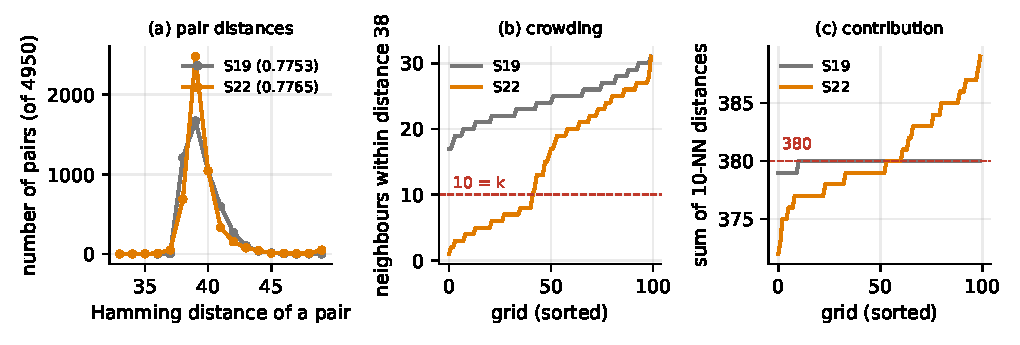
\includegraphics[width=0.95\linewidth]{fig4_distances.pdf}
\caption{S19 (grey) against the final set S22 (orange). (a) Distances between all pairs of layouts; the fixed core removes pairs at distance 37--38. (b) Number of other layouts within distance 38 of each layout: the 49 core layouts have 6.6 such neighbours on average (the other 51 have 22.9), so most of them sit under the limit $k=10$. (c) Each layout's contribution; 380 is the value when all ten neighbours are at 38.}
\label{fig:dist}
\end{figure}

\begin{figure}[h]
\centering
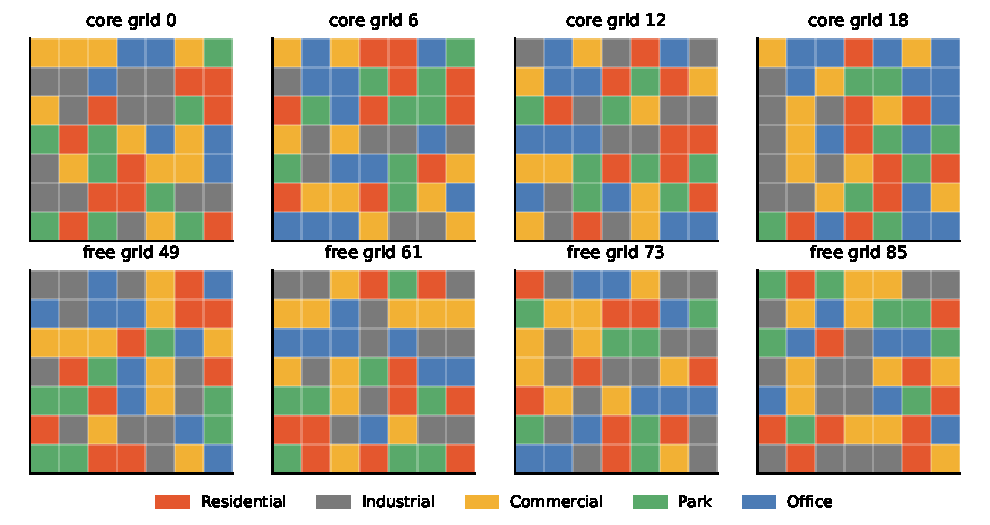
\includegraphics[width=0.6\linewidth]{fig3_grids.pdf}
\caption{Eight of the 100 layouts in S22: four from the fixed core (top) and four from the freely annealed part (bottom).}
\end{figure}

\begin{figure}[h]
\centering
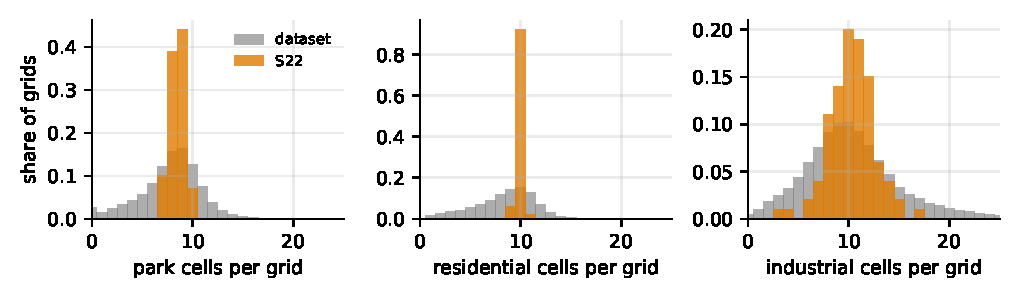
\includegraphics[width=0.9\linewidth]{fig5_composition.pdf}
\caption{Number of park, residential and industrial cells per layout, for a 10\% sample of the dataset and for S22. Valid layouts lie in a narrow band of compositions (almost every S22 layout has exactly 10 residential cells), which is why diversity has to come from \emph{where} the districts are placed, not from how many there are.}
\label{fig:comp}
\end{figure}

\begin{table}[h]
\centering
\small
\begin{tabular}{llcc}
\toprule
Set & Method & Score & Status \\
\midrule
S1 & layouts from the data & 0.3137 & returned \\
S2 & generated layouts & 0.6329 & returned \\
S8 & surrogate models, annealed set & 0.7540 & returned, 100/100 valid \\
S18 & exact rules, C++ annealer & 0.7734 & returned \\
S19 & exact rules, warm chains & 0.7753 & returned (matched prediction) \\
S21 & cold polish of a record set & 0.7754 & built, held back \\
\textbf{S22} & \textbf{fixed code core + hot chain} & \textbf{0.7765} & \textbf{final, all 100 valid} \\
\bottomrule
\end{tabular}
\caption{Selected submissions. S22 was checked with the exact Python rules (sha b2cb6b36).}
\end{table}

\section{What we learned}

\textbf{Look at the labels before choosing a model.} The ties and the $k/999$ spacing were visible in a histogram from day one, and noticing them did more than any change of model family. We spent two days improving surrogates by a percent or two before we asked why the labels looked the way they did.

\textbf{A plateau is a hint about a wrong assumption.} Every model, whatever its architecture, stopped at the same error. The cause was a symmetry we had assumed instead of tested, and a single check (split the adjacency terms by direction) removed it. The faster experiment would have been to submit a rotated copy of a certified set on day one.

\textbf{Treat submissions as measurements.} A returned score tells you how many layouts failed, so probes made of a certified set plus a few risky layouts answered questions that the training data could not.

\textbf{Exact beats confident.} Once the rules were exact, no submission lost a layout. We also checked the C++ annealer against the Python rules on 22{,}000 layouts, because a bug there would have silently invalidated everything.

\textbf{Understand the ceiling, then use structure.} Knowing why annealing stalls at 38000 led to the coding-theory idea, which beat every set annealed from scratch. The first fixed-core runs looked like a failure only because the temperature was too low, so a negative result can just mean a bad setting.

\textbf{Run the cluster carefully.} Resumable jobs mattered more than raw speed. We also lost time by editing a script while a job was still running it, and we lowered our own priority with a few heavy days of 96-core runs.

\section{Future work}

\begin{itemize}
\item \textbf{More valid code layouts.} The core was the biggest single lever (each core layout is worth about 5 points over a free one), and we only managed 49 of 125. An exact method (integer programming or SAT over the arrangement and relabelling), or a different code, could raise this and with it the ceiling of $0.796$.
\item \textbf{Longer, tuned runs.} The final chains were still improving when their jobs ended. We prepared an overnight run of 96 restarting chains, but did not launch it. Parallel tempering across cores is another option.
\item \textbf{A bound.} We have no idea how far above $0.7765$ the true optimum is. A relaxation of the packing problem under the exact validity region would tell us whether more effort is worthwhile.
\item \textbf{Automate the rule discovery.} Look at the label distribution, recover the integer target, fit sparse count, distance and directional terms, and accept a fit only if it is exact. This could be written as symbolic regression with exactness as the stopping test, and would apply to any discrete black-box scorer.
\end{itemize}

\section*{Acknowledgement of AI use}
We used Claude Code (Anthropic, model Claude Sonnet 5.5, Opus 5.5, Fable 5.2) as a coding and writing assistant throughout this project. It helped write and run code and the write first draft of this report. We chose the directions, made the submission decisions, and uploaded every file ourselves. The final scores quoted here come from the leaderboard or from the exact scoring code in the repository, not from the assistant's own estimates.

\textbf{Code.} The exact rules are in \texttt{src/rules.py}, the annealer in \texttt{src/anneal.cpp}, and the day-by-day log and every submission with its predicted and returned score are in \texttt{UPDATES.md} and \texttt{results/submission\_log.jsonl}.

\end{document}
